\begin{figure*}[hbtp]
  \centering
  % \includegraphics[width=0.44\linewidth]{out/8020-speedup-key.pdf}
  \subfigure[Overall result]{
    \label{fig:8020-speedup--mean}
    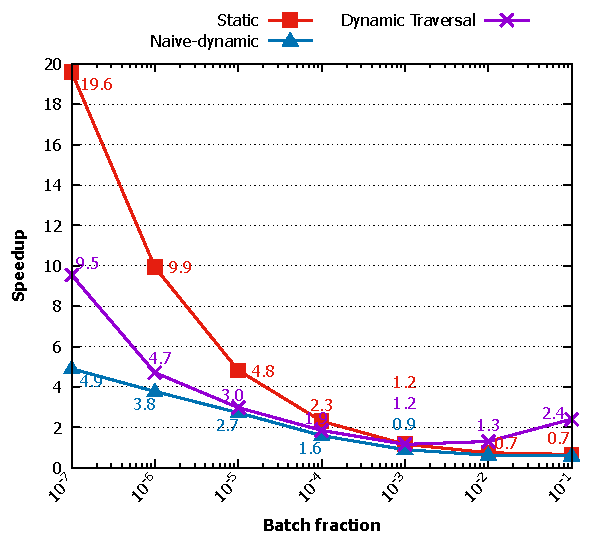
\includegraphics[width=0.38\linewidth]{out/8020-speedup-mean.pdf}
  }
  \subfigure[Results on each graph]{
    \label{fig:8020-speedup--all}
    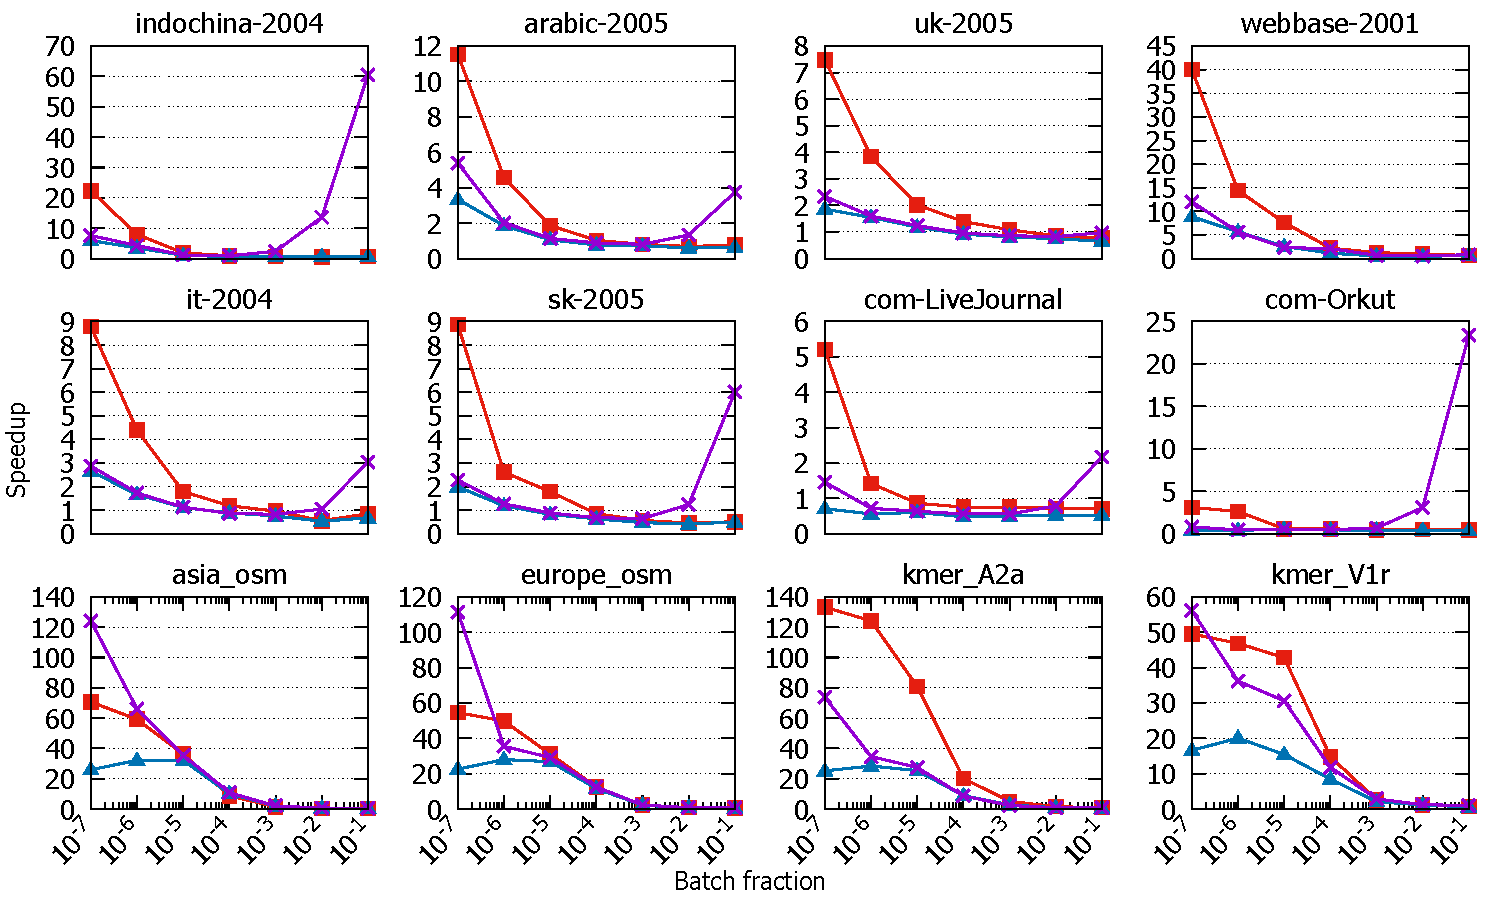
\includegraphics[width=0.58\linewidth]{out/8020-speedup-all.pdf}
  } \\[-1ex]
  \caption{Speedup of \textit{Dynamic Frontier} PageRank with respect to \textit{Static}, \textit{Naive-dynamic}, and \textit{Dynamic Traversal} PageRank on batch updates of size $10^{-7} |E|$ to $0.1 |E|$ (logarithmic scale), with $80\%$ edge insertions and $20\%$ edge deletions --- representing a realistic batch update upon a dynamic graph. The figure on the right shows the speedup of \textit{Dynamic Frontier} PageRank, with respect to each approach, for each graph in the dataset --- while the figure of the left highlights the overall speedup.}
  \label{fig:8020-speedup}
\end{figure*}
